%Aufbau
\section{Aufbau}
\subsection{Architektur}
Grundsätzlich teilt sich \softwarename in zwei Hauptbestandteile auf.
Es wird ein Backend- und ein Frontend-Bestandteil implementiert.
Das Frontend läuft als Java-Script im Browser des Nutzers und ist für die Anzeige und Visualisierung der Daten, sowie den Bau der Oberfläche verantwortlich.
Das Backend wird als in Java implementierte Spring-Boot-Anwendung auf einem Server ausgeführt.
Dieses Anwendungsframework ermöglicht es in Java die \gls{RESTAPI} einer Sensorthingsdatenbank abzufragen.
\\
Grundsätzlich lässt sich der Aufbau also wie folgt darstellen.
\\
\begin{figure} [h]
    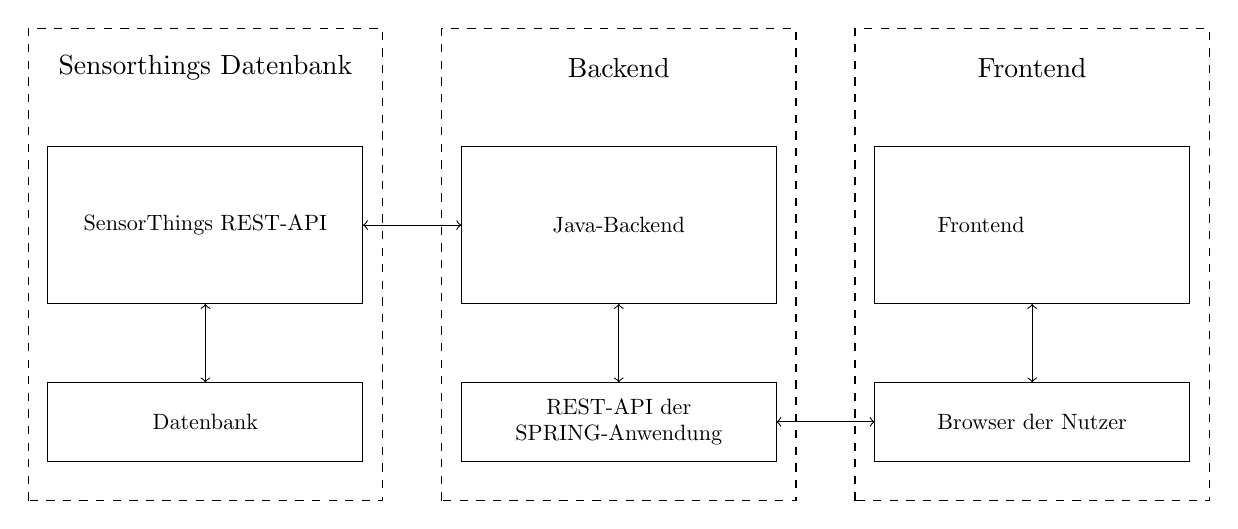
\begin{tikzpicture}[node distance=2cm]

        %Model
        \begin{scope}[shift={(0,0)},local bounding box=SensorThings]
            \draw (0,0) [dashed] rectangle (4.5,6);
            \node[scale=1] at (2.25,5.5) {Sensorthings Datenbank};
            \begin{scope}[local bounding box=API]
                \draw (0.25,2.5) rectangle (4.25,4.5);
                \node[scale=0.8] at (2.25,3.5) {SensorThings REST-API};
            \end{scope}
            \begin{scope}[local bounding box=Datenbank]
                \draw (0.25,0.5) rectangle (4.25,1.5);
                \node[scale=0.8] at (2.25,1) {Datenbank};
            \end{scope}
        \end{scope}
        
        %Controller
        \begin{scope}[shift={(5.25,0)},local bounding box=Backend]
            \draw (0,0) [dashed] rectangle (4.5,6);
            \node[scale=1] at (2.25,5.5) {\softwarename Backend};
            \begin{scope}[local bounding box=VisAQBackend]
                \draw (0.25,2.5) rectangle (4.25,4.5);
                \node[scale=0.8] at (2.25,3.5) {\softwarename Java-Backend};
            \end{scope}
            \begin{scope}[local bounding box=BackendAPI]
                \draw (0.25,0.5) rectangle (4.25,1.5);
                \node[scale=0.8, align=center] at (2.25,1) {REST-API der\\SPRING-Anwendung};
            \end{scope}
        \end{scope}

        %View
        \begin{scope}[shift={(10.5,0)},local bounding box=Frontend]
            \draw (0,0) [dashed] rectangle (4.5,6);
            \node[scale=1] at (2.25,5.5) {\softwarename Frontend};

            \begin{scope}[local bounding box=VisAQFrontend]
                \draw (0.25,2.5) rectangle (4.25,4.5);
                \node[scale=0.8,text width=3cm] at (2.25,3.5) {\softwarename Frontend};
            \end{scope}
            \begin{scope}[local bounding box=Browser]
                \draw (0.25,0.5) rectangle (4.25,1.5);
                \node[scale=0.8] at (2.25,1) {Browser der Nutzer};
            \end{scope}
        \end{scope}

        \draw[<->] (API.south) -- (Datenbank.north);
        \draw[<->] (API.east) -- (VisAQBackend.west);
        \draw[<->] (BackendAPI.north) -- (VisAQBackend.south);
        \draw[<->] (BackendAPI.east) -- (Browser.west);
        \draw[<->] (VisAQFrontend.south) -- (Browser.north);

    \end{tikzpicture}
    \caption{Diagramm des Gesamt-Systems}
\end{figure}
\\
Alle drei großen Komponenten können hierbei auf verschiedenen Geräten liegen und kommunizieren über die REST-API miteinander.
Durch die Softwarekombination \softwarename werden lediglich die beiden Komponenten \softwarename Backend und \softwarename Frontend bereitgestellt.
\\
Beide Softwarekomponenten sind nach dem \gls{MVC}-Entwurfsmuster aufgebaut.
\subsubsection{Backend}
Das Backend wird als Spring-Boot-Anwendung (\url{https://spring.io/projects/spring-boot}) ausgeführt.
Diese Softwarekomponente besitzt keinen dem MVC-Entwurfsmuster entsprechenden Viewanteil, da im Backend keine Anzeige stattfindet.
\\
Das System baut sich wie folgt auf:
\\
\begin{figure} [h]
    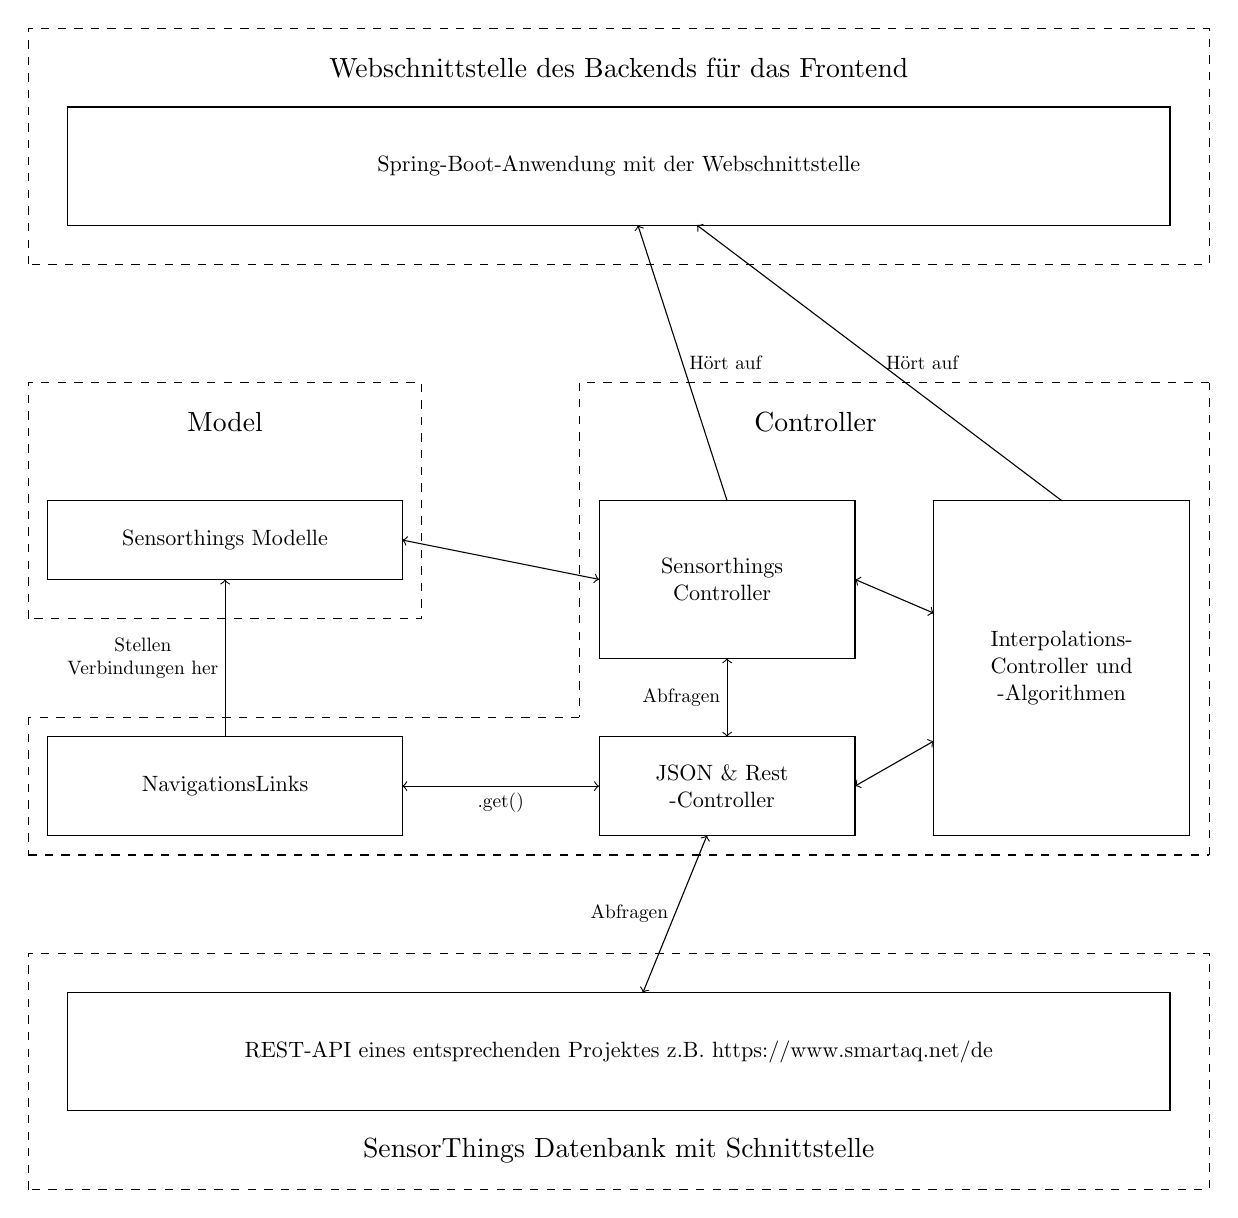
\begin{tikzpicture}[node distance=2cm]

        %SPRING
        \begin{scope}[shift={(0,11.75)},local bounding box=SPRING]
            \draw (0,0) [dashed] rectangle (15,3);
            \node[scale=1] at (7.5,2.5) {Webschnittstelle des Backends für das Frontend};
            \begin{scope}[local bounding box=SPRINGWEB]
                \draw (0.5,0.5) rectangle (14.5,2);
                \node[scale=0.8, align=center] at (7.5,1.25) {Spring-Boot-Anwendung mit der Webschnittstelle};
            \end{scope}
        \end{scope}

        %Model
        \begin{scope}[shift={(0,4.25)},local bounding box=SensorThings]
            \draw (0,3) [dashed] rectangle (5,6);
            \node[scale=1] at (2.5,5.5) {Model};
            \begin{scope}[local bounding box=SensorthingsM]
                \draw (0.25,3.5) rectangle (4.75,4.5);
                \node[scale=0.8] at (2.5,4) {Sensorthings Modelle};
            \end{scope}
            \begin{scope}[local bounding box=Link]
                \draw (0.25,0.25) rectangle (4.75,1.5);
                \node[scale=0.8] at (2.5,.875) {NavigationsLinks};
            \end{scope}
        \end{scope}

        %Controller
        \begin{scope}[shift={(7,4.25)},local bounding box=Backend]
            %\draw (0,0) [dashed] rectangle (8,6);
            \draw [dashed] (-7,0) -- (8,0);
            \draw [dashed] (8,0) -- (8,6);
            \draw [dashed] (8,6) -- (0,6);
            \draw [dashed] (0,6) -- (0,1.75);
            \draw [dashed] (0,1.75) -- (-7,1.75);
            \draw [dashed] (-7,1.75) -- (-7,0);
            \node[scale=1] at (3,5.5) {Controller};
            \begin{scope}[local bounding box=STController]
                \draw (0.25,2.5) rectangle (3.5,4.5);
                \node[scale=0.8,align=center] at (1.8125,3.5) {Sensorthings\\Controller};
            \end{scope}
            \begin{scope}[local bounding box=JSONREST]
                \draw (0.25,0.25) rectangle (3.5,1.5);
                \node[scale=0.8, align=center] at (1.8125,.875) {JSON \& Rest\\-Controller};
            \end{scope}
            \begin{scope}[local bounding box=Interpolation]
                \draw (4.5,0.25) rectangle (7.75,4.5);
                \node[scale=0.8, align=center] at (6.125,2.375) {Interpolations-\\Controller und\\-Algorithmen};
            \end{scope}
        \end{scope}

        %Sensorthings Datenbank
        \begin{scope}[shift={(0,0)},local bounding box=Backend]
            \draw (0,0) [dashed] rectangle (15,3);
            \node[scale=1] at (7.5,0.5) {SensorThings Datenbank mit Schnittstelle};
            \begin{scope}[local bounding box=SensorthingsAPI]
                \draw (0.5,1) rectangle (14.5,2.5);
                \node[scale=0.8, align=center] at (7.5,1.75) {REST-API eines entsprechenden Projektes z.B. https://www.smartaq.net/de};
            \end{scope}
        \end{scope}

        \draw[->] (Link.north) -- (SensorthingsM.south) node[midway,left,scale=0.7,align=center] {Stellen\\Verbindungen her};
        \draw[<->] (SensorthingsAPI) -- (JSONREST) node[midway,left,scale=0.7,align=center] {Abfragen};
        \draw[<->] (Link.east) -- (JSONREST.west) node[midway,below,scale=0.7,align=center] {.get()};
        \draw[<->] (JSONREST.north) -- (STController.south) node[midway,left,scale=0.7,align=center] {Abfragen};
        \draw[<->] (SensorthingsM.east) -- (STController.west);
        \draw[<->] (Interpolation) -- (STController.east);
        \draw[<->] (Interpolation) -- (JSONREST.east);
        \draw[<-] (SPRINGWEB) -- (Interpolation.north) node[midway,right,scale=0.7,align=center] {Hört auf};
        \draw[<-] (SPRINGWEB) -- (STController.north) node[midway,right,scale=0.7,align=center] {Hört auf};
    \end{tikzpicture}
    \caption{Aufbau des \softwarename Backends}
\end{figure}

\\
Im Folgenden sollen kurz die einzelnen Bestandteile erläutert werden.
\begin{itemize}
    \item \textbf{SensorThings Datenbank mit Schnittstelle} Diese Datenbankschnittstelle wird nicht von \softwarename implementiert, sondern wird von einem Projekt wie zum Beispiel SmartAQnet bereitgestellt und ist zwingend nötig für den Betrieb der Software.
    \item \textbf{Model} Im Model werden alle Objekte der SensorThings-API nachimplementiert.
    \item \textbf{Controller} Im Controller werden alle in der Webschnittstelle verfügbaren Funktionen implementiert.
    Durch das Mapping der verschiedenen Funktionen unter Verwendung des Spring-Framework werden Funktionen der Controller von außen erreichbar.
    \item \textbf{Webschnittstelle} Die Webschnittstelle des Backends wird von der Spring-Boot-Anwendung bereitgestellt.
\end{itemize}
\clearpage
\subsubsection{Frontend}
Das Frontend beinhaltet alle drei Komponenten des \gls{MVC}-Entwurfsmusters. Die angezeigten Messdaten bezieht das \softwarename Frontend ausschließlich vom \softwarename Backend
Im Frontend wird der Java Transpiler \gls{Jsweet} verwendet. Zur Darstellung wird das \gls{Angular-4-Candy} für \gls{Jsweet} verwendet.
Das System baut sich wie folgt auf:
\\
\begin{figure} [h]
    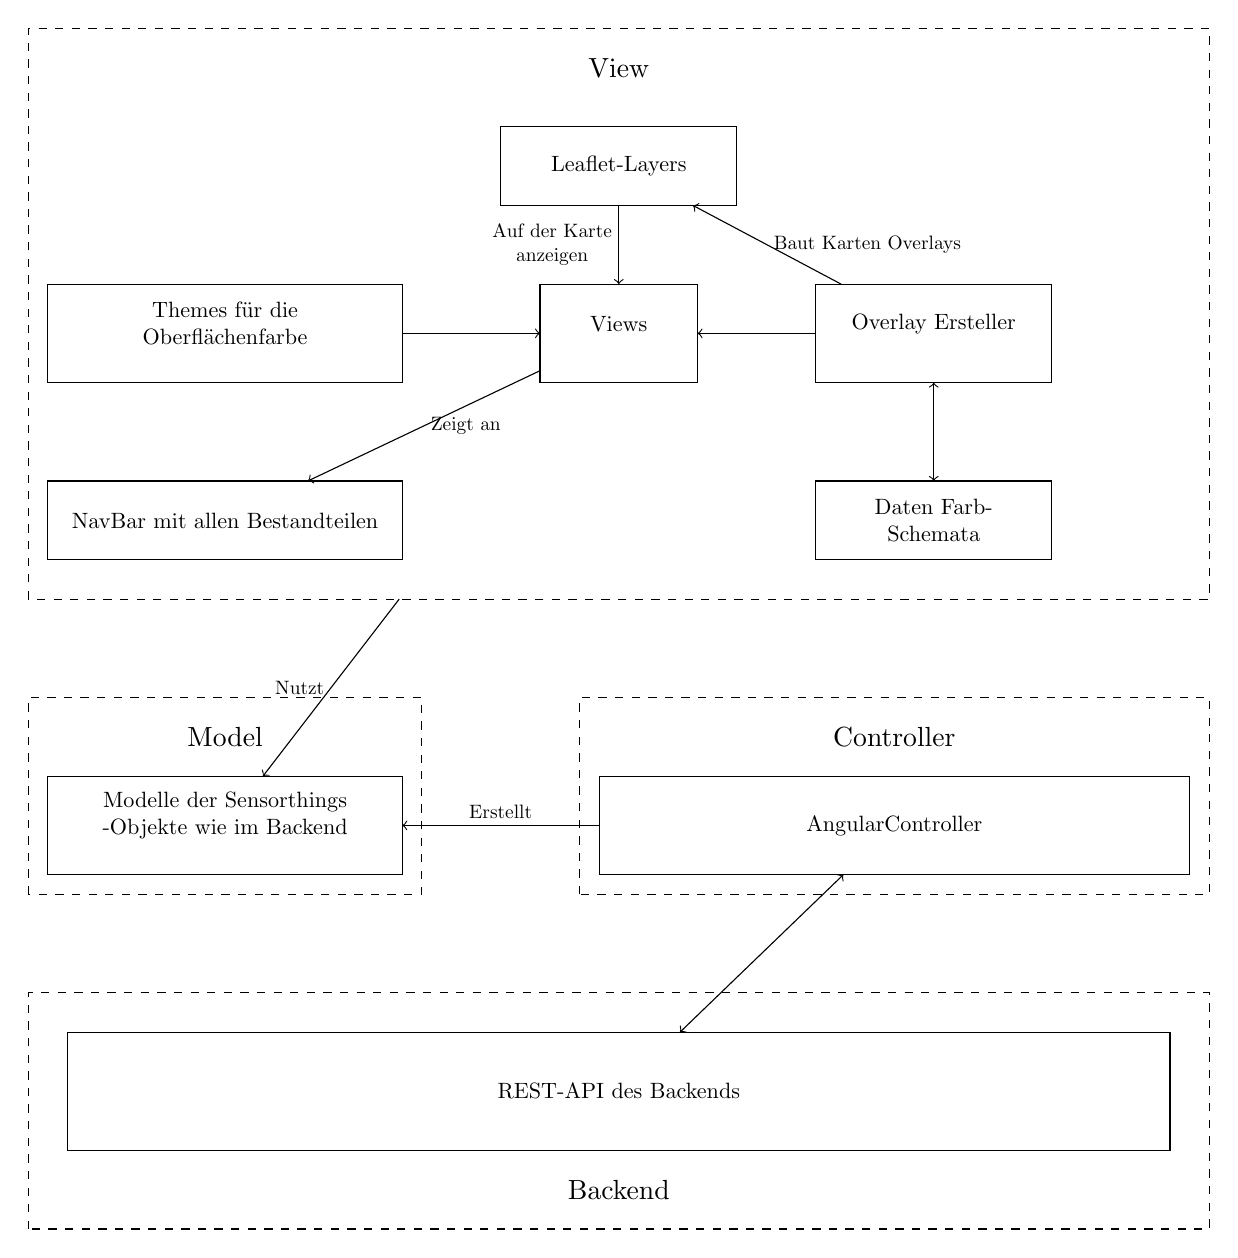
\begin{tikzpicture}[node distance=2cm]

        %View
        \begin{scope}[shift={(0,8)},local bounding box=View]
            \draw (0,0) [dashed] rectangle (15,7.25);
            \node[scale=1] at (7.5,6.75) {View};
            \begin{scope}[local bounding box=Themes]
                \draw (0.25,2.75) rectangle (4.75,4);
                \node[scale=0.8,align=center] at (2.5,3.5) {Themes für die\\Oberflächenfarbe};
            \end{scope}
            \begin{scope}[local bounding box=Views]
                \draw (6.5,2.75) rectangle (8.5,4);
                \node[scale=0.8,align=center] at (7.5,3.5) {Views};
            \end{scope}
            \begin{scope}[local bounding box=Leaflet]
                \draw (6,5) rectangle (9,6);
                \node[scale=0.8,align=center] at (7.5,5.5) {Leaflet-Layers};
            \end{scope}
            \begin{scope}[local bounding box=OverlayBuilder]
                \draw (10,2.75) rectangle (13,4);
                \node[scale=0.8,align=center] at (11.5,3.5) {Overlay Ersteller};
            \end{scope}
            \begin{scope}[local bounding box=NavBar]
                \draw (0.25,1.5) rectangle (4.75,.5);
                \node[scale=0.8,align=center] at (2.5,1) {NavBar mit allen Bestandteilen};
            \end{scope}
            \begin{scope}[local bounding box=aqd]
                \draw (10,1.5) rectangle (13,.5);
                \node[scale=0.8,align=center] at (11.5,1) {Daten Farb-\\Schemata};
            \end{scope}
        \end{scope}

        %Model
        \begin{scope}[shift={(0,4.25)},local bounding box=Model]
            \draw (0,0) [dashed] rectangle (5,2.5);
            \node[scale=1] at (2.5,2) {Model};
            \begin{scope}[local bounding box=STM]
                \draw (0.25,0.25) rectangle (4.75,1.5);
                \node[scale=0.8,align=center] at (2.5,1) {Modelle der Sensorthings\\-Objekte wie im Backend};
            \end{scope}
        \end{scope}
        
        %Controller
        \begin{scope}[shift={(7,4.25)},local bounding box=Controller]
            \draw (0,0) [dashed] rectangle (8,2.5);
            \node[scale=1] at (4,2) {Controller};
            \begin{scope}[local bounding box=ACon]
                \draw (0.25,0.25) rectangle (7.75,1.5);
                \node[scale=0.8, align=center] at (4,.875) {AngularController};
            \end{scope}
        \end{scope}

        %Backend
        \begin{scope}[shift={(0,0)},local bounding box=Backend]
            \draw (0,0) [dashed] rectangle (15,3);
            \node[scale=1] at (7.5,0.5) {\softwarename Backend};
            \begin{scope}[local bounding box=RESTAPI]
                \draw (0.5,1) rectangle (14.5,2.5);
                \node[scale=0.8, align=center] at (7.5,1.75) {REST-API des \softwarename Backends};
            \end{scope}
        \end{scope}

        \draw[->] (View) -- (STM) node[midway,left,scale=0.7,align=center] {Nutzt};
        \draw[->] (ACon.west) -- (STM.east) node[midway,above,scale=0.7,align=center] {Erstellt};
        \draw[<->] (ACon) -- (RESTAPI);
        \draw[->] (Leaflet) -- (Views) node[midway,left,scale=0.7,align=center] {Auf der Karte\\anzeigen};
        \draw[->] (Themes) -- (Views);
        \draw[->] (OverlayBuilder) -- (Views);
        \draw[->] (OverlayBuilder) -- (Leaflet) node[midway,right,scale=0.7,align=center] {Baut Karten Overlays};
        \draw[->] (Views) -- (NavBar) node[midway,right,scale=0.7,align=center] {Zeigt an};
        \draw[<->] (aqd) -- (OverlayBuilder);
    \end{tikzpicture}
    \caption{Aufbau des \softwarename Frontends}
\end{figure}
\\
Im Folgenden sollen kurz die einzelnen Bestandteile erläutert werden.
\begin{itemize}
    \item \textbf{VisAQ Backend} Das \softwarename Backend wird hier für die Besorgung der angezeigten Daten verwendet. Es läuft als Spring-Boot-Anwendung auf einem Server.
    \item \textbf{Model} Im Model werden alle Objekte der \gls{SensorThings API} nachimplementiert, die auch im Backend existieren.
    Die Implementierung der Model-Klassen ist jedoch im Gegensatz zum Backend stark vereinfacht, da große Teile der Logik hier nicht benötigt werden.
    \item \textbf{Controller} Der Controller besteht hier aus einer Klasse, die die Logik des Angular-Paketes nutzt, um mit dem Backend zu kommunizieren.
    \item \textbf{View} Die View baut mit verschiedenen Factories und Elementen Oberflächen zusammen, die im Browser des Nutzers angezeigt werden.
\end{itemize}

\subsection{Klassendiagramm}
\subsection{Backend}
\clearpage
\begin{figure} [h]
    \begin{adjustbox}{addcode={\begin{minipage}{\width}}{\caption{%
        Klassen-Diagramm des Backend (\url{http://visaq.de/files/Backend_final.png})
        }\end{minipage}},rotate=90,center}
        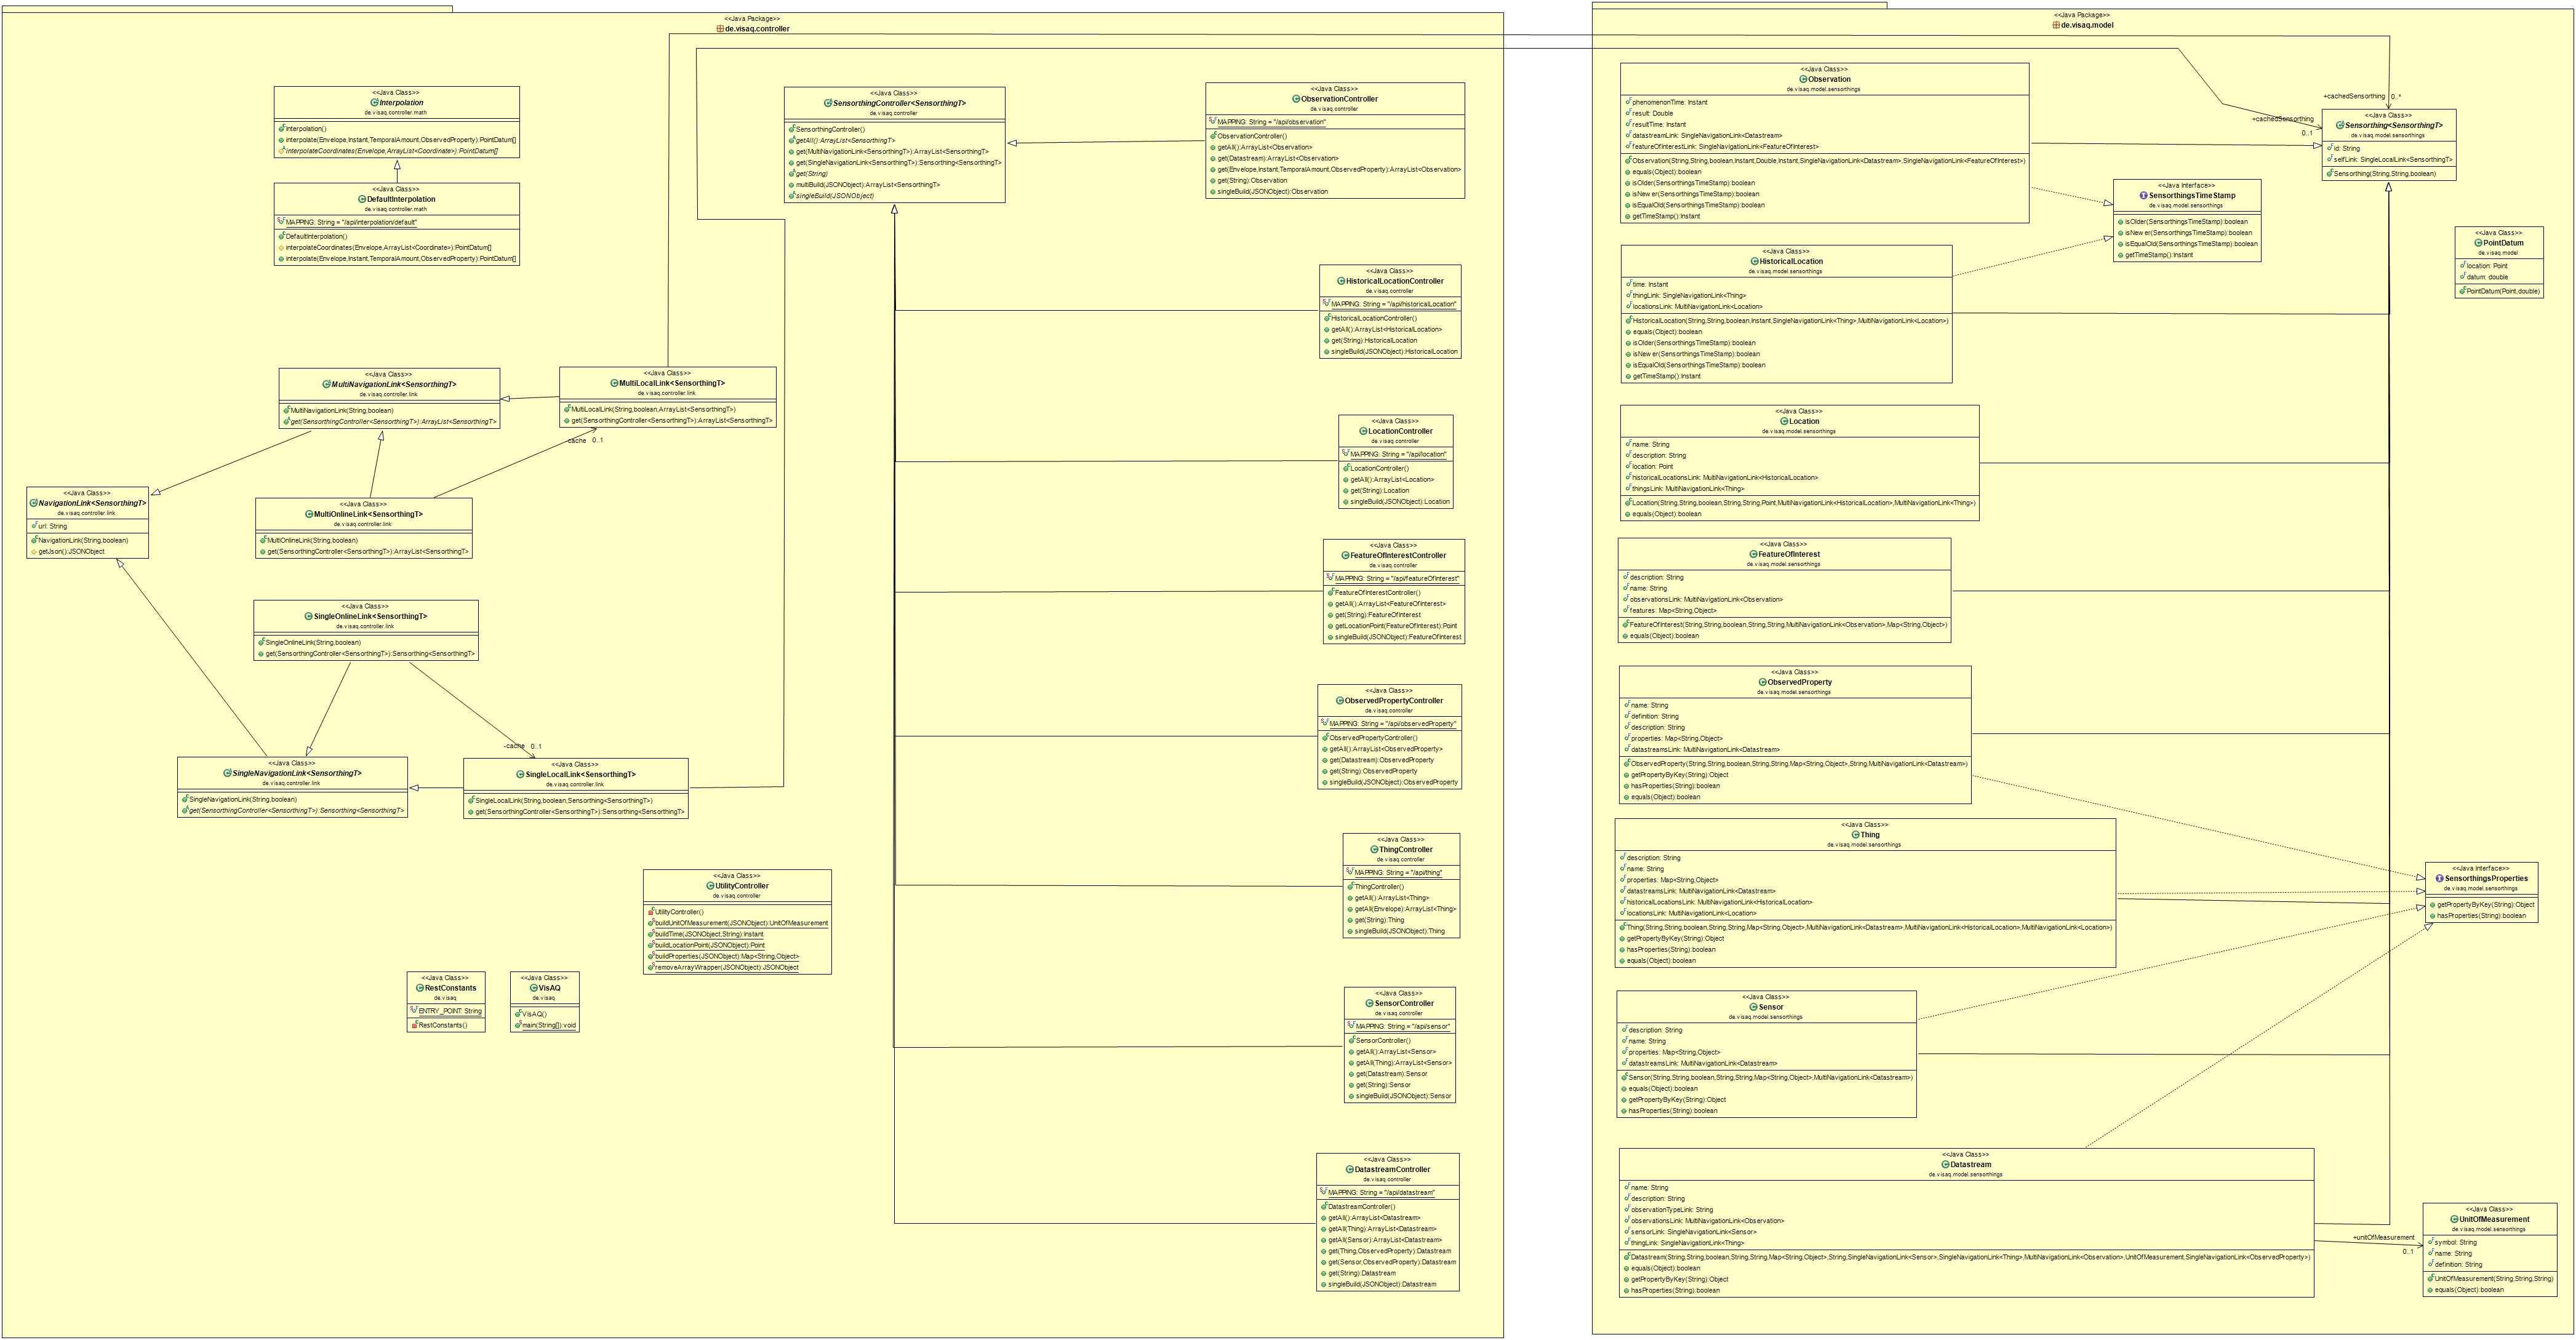
\includegraphics[height=0.75\textwidth]{media/backend/Backend.png}
    \end{adjustbox}
\end{figure}
\clearpage
\begin{figure} [h]
	\subsection{Frontend}
   	\begin{adjustbox}{addcode={\begin{minipage}{\width}}{\caption{%
   		Klassen-Diagramm des Frontend (\url{http://visaq.de/files/Frontend_final.png})
   		}\end{minipage}},rotate=90,center}
   		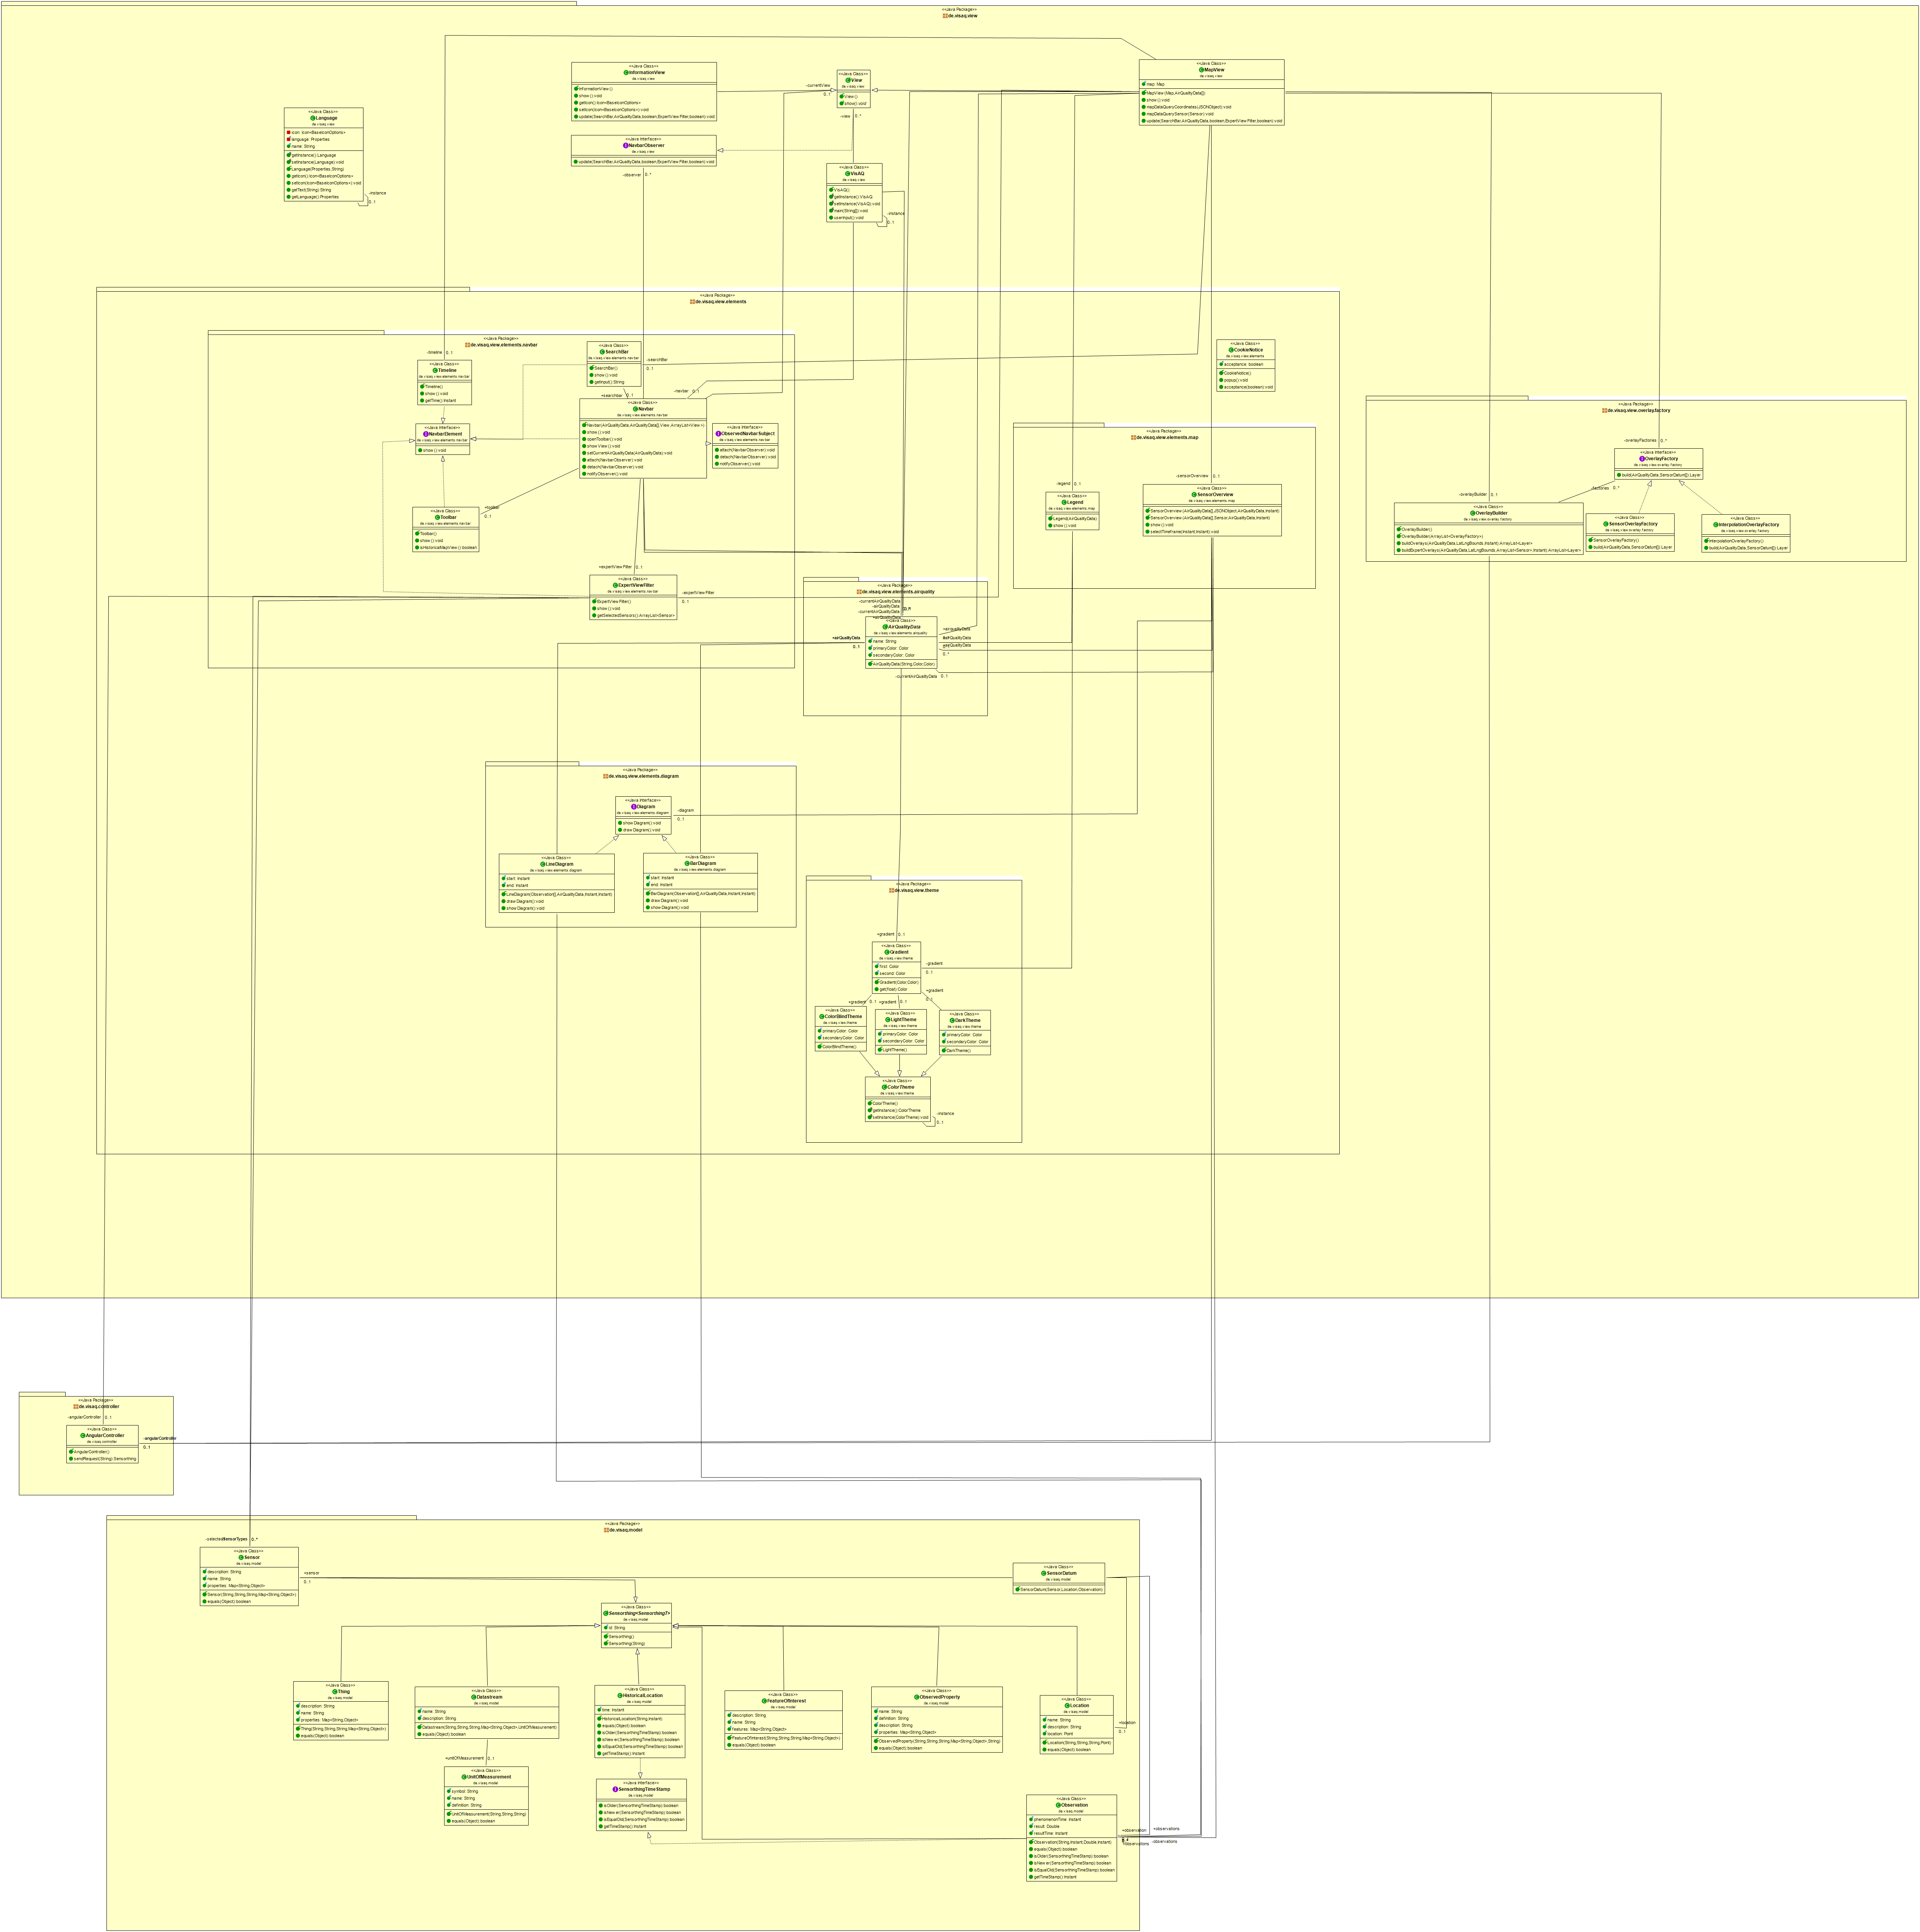
\includegraphics[height=0.7\textwidth]{media/frontend/frontend.png}
   	\end{adjustbox}
\end{figure}
\clearpage